\lhead[\thepage]{APÉNDICE B. MANUAL DE USUARIO}
\chead[]{}
\rhead[WepSIM: Simulador de un procesador elemental con unidad de control microprogramada]{\thepage}
\renewcommand{\headrulewidth}{0.5pt}

\lfoot[]{}
\cfoot[]{}
\rfoot[]{}
\renewcommand{\footrulewidth}{0pt}




\chapter{Manual de usuario}
\label{ch:apendiceb}


Este anexo presenta un manual de usuario detallado de WepSIM. En primer lugar, se indica el ciclo de ejecución en el simulador, explicando la gestión del microcódigo, el código ensamblador y la realización de una simulación. Después, se indica el formato de definición del microcódigo. Tras ello, se indica el formato del código ensamblador. Por último, se indica la definición de un juego de instrucciones y un código ensamblador base.

\section*{Ejecución en WepSIM}

El ciclo de trabajo para el usuario en WepSIM supone (normalmente) los siguientes pasos:

\begin{itemize}

\item Cargar un juego de instrucciones de trabajo.

\item Cargar un programa en ensamblador que utilice el juego de instrucciones de trabajo.

\item Ir a la pantalla principal del simulador para realizar la ejecución del programa ensamblador que utilice el juego de instrucciones de trabajo.

\end{itemize}

\subsection*{Gestión de microcódigo en WepSIM}
\label{ch:anexob_microcodigo}

Un fichero de texto con las tres secciones antes comentadas (microcódigo, nombrado de registro y definición de pseudo-instrucciones) se carga en la pantalla de Firmware. Para acceder a dicha pantalla se ha de ir al menú (parte superior derecha) e indicar la opción Firmware (Figura \ref{fig:anexob-1}).

\begin{figure}[htbp]
 	\centering
 	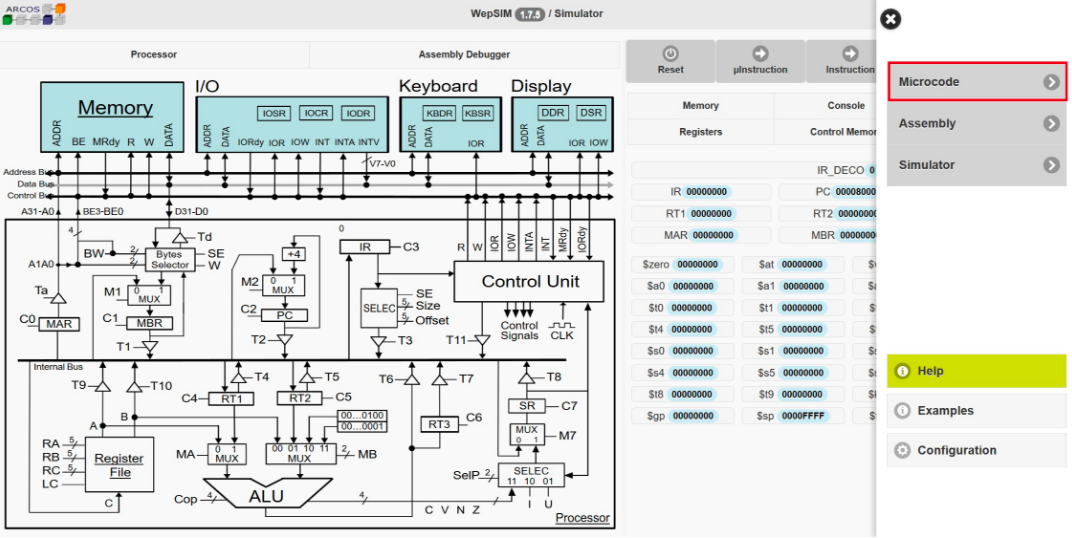
\includegraphics[width=15cm]{figures/anexob-1}
 	\caption{Pantalla principal: opción de carga de juego de firmware.}
	\label{fig:anexob-1}
\end{figure}

A continuación aparecerá una pantalla con un cuadro de texto que permite indicar el firmware (las tres secciones antes comentadas). Es posible cargar un firmware existente usando el botón "Load" de la barra inferior, modificar un firmware anteriormente cargado o salvar el firmware en curso con el botón ``Save'' de la barra inferior. Una vez se indique el firmware es preciso hacer clic en el botón ``micro-compile'' para pasar a binario y cargar en la memoria de control dicho firmware, como se muestra en la Figura \ref{fig:anexob-2}.

\begin{figure}[htbp]
 	\centering
 	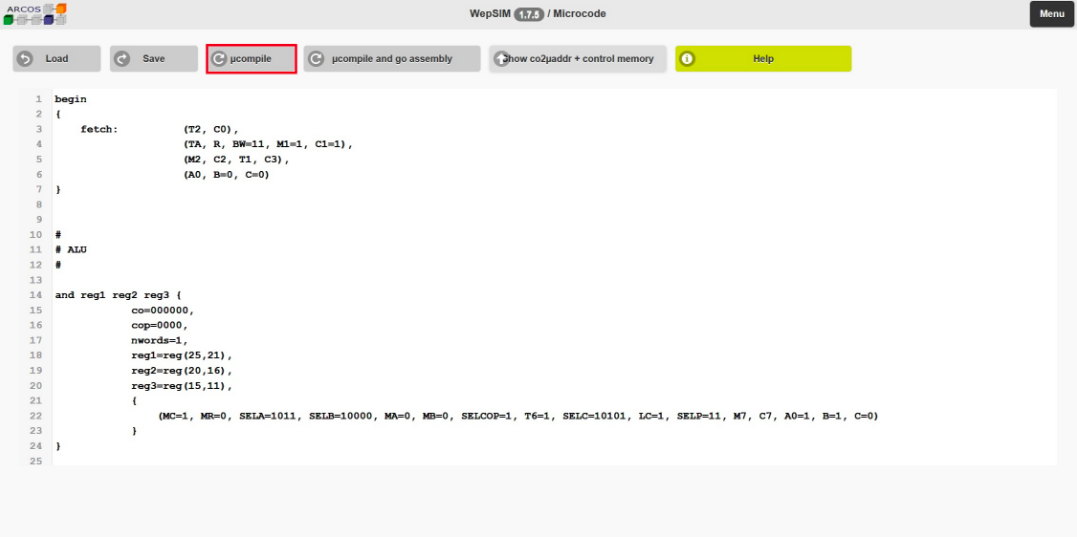
\includegraphics[width=15cm]{figures/anexob-2}
 	\caption{Pantalla firmware: cuadro de texto con firmware a cargar.}
	\label{fig:anexob-2}
\end{figure}

Una vez cargado el nuevo firmware correctamente aparecerá la pantalla mostrada en la Figura \ref{fig:anexob-3} en la que se muestra la memoria de control con los valores que almacena.

\begin{figure}[htbp]
 	\centering
 	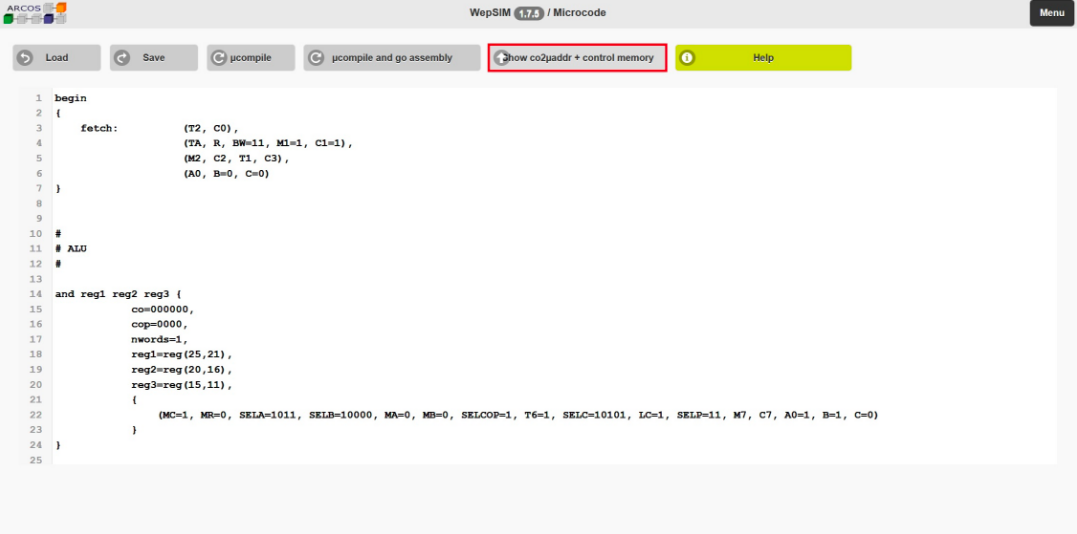
\includegraphics[width=15cm]{figures/anexob-3}
 	\caption{Pantalla firmware: firmware finalmente compilado.}
	\label{fig:anexob-3}
\end{figure}

El siguiente paso es la carga del programa ensamblador que permita probar este firmware, para ello podemos pulsar el botón ``Assembly'' de la barra inferior.

\subsection*{Gestión de código ensamblador en WepSIM}
\label{ch:anexob_assembly}

Un fichero de texto con las dos secciones antes comentadas (datos y código) se carga en la pantalla de Ensamblador. Para acceder a dicha pantalla se ha de ir al menú (parte superior derecha) e indicar la opción Assembly (\ref{fig:anexob-4}).

A continuación aparecerá una pantalla con un cuadro de texto que permite indicar el código en ensamblador. Es posible cargar un código existente usando el botón "Load" de la barra superior, modificar un código anteriormente cargado o salvar el código actualmente en cargado con el botón ``Save'' de la barra inferior.

\begin{figure}[htbp]
 	\centering
 	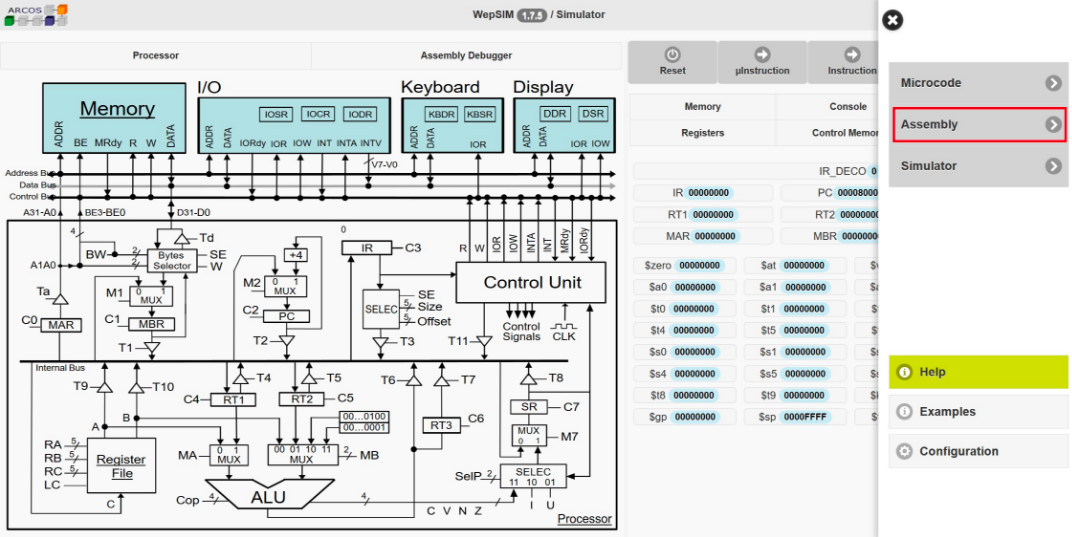
\includegraphics[width=15cm]{figures/anexob-4}
 	\caption{Pantalla principal: opción de carga de código ensamblador.}
	\label{fig:anexob-4}
\end{figure}
Una vez se indique el código es preciso hacer clic en el botón "Compile" para pasar a binario y cargar en la memoria de principal el binario resultante, tal y como se muestra en la Figura \ref{fig:anexob-5}.

\begin{figure}[htbp]
 	\centering
 	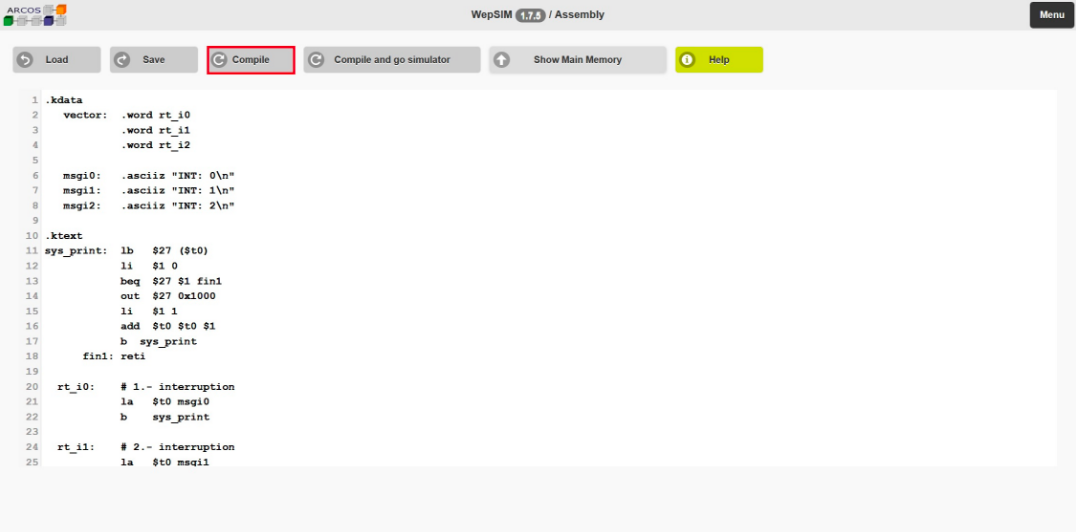
\includegraphics[width=15cm]{figures/anexob-5}
 	\caption{Pantalla ensamblador: cuadro de texto con ensamblador a cargar.}
	\label{fig:anexob-5}
\end{figure}

Una vez compilado, se pasará a la pantalla indicada en la Figura \ref{fig:anexob-6} donde se mostrará el contenido de la memoria principal en binario.

\begin{figure}[htbp]
 	\centering
 	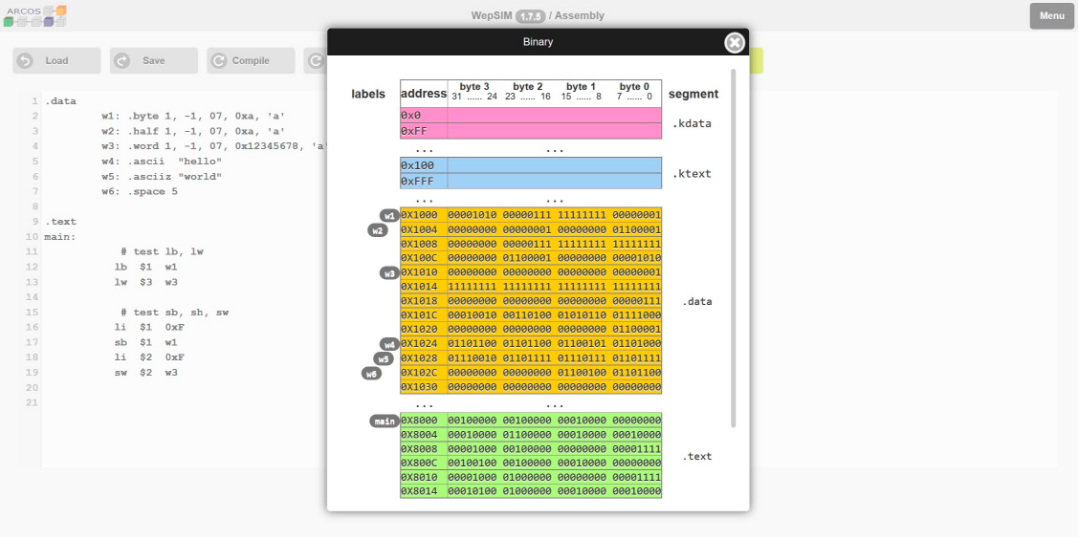
\includegraphics[width=15cm]{figures/anexob-6}
 	\caption{Pantalla ensamblador: código finalmente compilado.}
	\label{fig:anexob-6}
\end{figure}
El siguiente paso es ir a la pantalla principal para ejecutar la combinación de firmware y ensamblador cargado, para lo que ha de pulsar el botón "Simulador" de la barra inferior.

\subsection*{Simulación en WepSIM}
\label{ch:anexob_simulacion}

Estando en la pantalla principal es posible visualizar:

\begin{itemize}

\item El contenido de la memoria de control (Figura \ref{fig:anexob-7}), con las señales que están asociadas a cada ciclo. Para ello ha de pulsar el botón ``Control Memory'' en la barra de botones situada en la parte superior derecha de la pantalla principal.

\item Se destaca las señales que en el presente ciclo de reloj están activadas en azul con letra algo más grande.

\item Se dispone de una barra de desplazamiento para poder inspeccionar todo el contenido de la memoria de control.

\item El contenido de la memoria principal (Figura \ref{fig:anexob-8}), con las instrucciones en ensamblador a ejecutar. Para estas, es posible establecer un punto de ruptura haciendo clic en la columna breakpoints. Al establecer un punto de ruptura aparecerá un icono en dicha columna.

\end{itemize}

\begin{figure}[htbp]
 	\centering
 	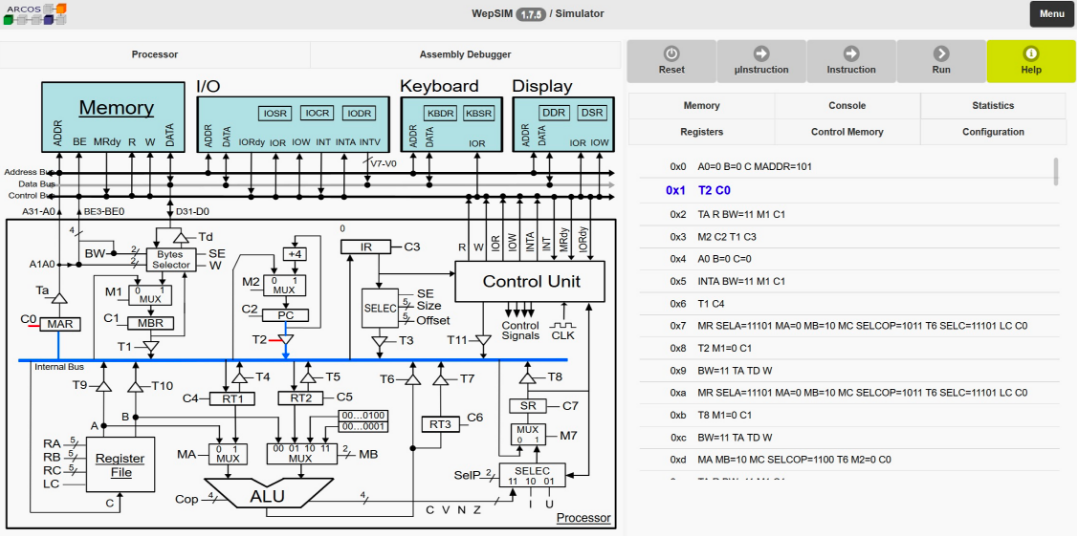
\includegraphics[width=15cm]{figures/anexob-7}
 	\caption{Pantalla principal: visualización de la memoria de control.}
	\label{fig:anexob-7}
\end{figure}

\begin{figure}[htbp]
 	\centering
 	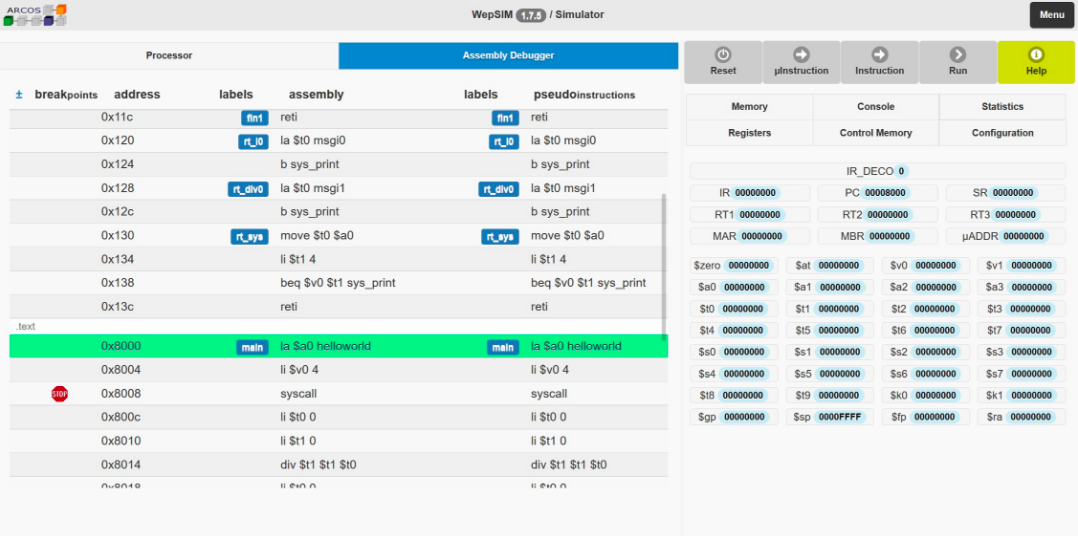
\includegraphics[width=15cm]{figures/anexob-8}
 	\caption{Pantalla principal: visualización del código en la memoria principal.}
	\label{fig:anexob-8}
\end{figure}

Estando en la pantalla principal es posible ejecutar:

\begin{itemize}

\item Microinstrucción a microinstrucción pulsando el botón ``micro-Instrucción'' (Figura \ref{fig:anexob-9}), de forma que se pasará al siguiente ciclo de reloj y se generarán las señales de control asociadas.

\item Instrucción a instrucción pulsando el botón ``Instrucción'' (Figura 26 \ref{fig:anexob-9}) de forma que se generarán todos los ciclos de reloj asociados al microprograma de la instrucción, parando al principio del fetch.

\end{itemize}

\begin{figure}[htbp]
 	\centering
 	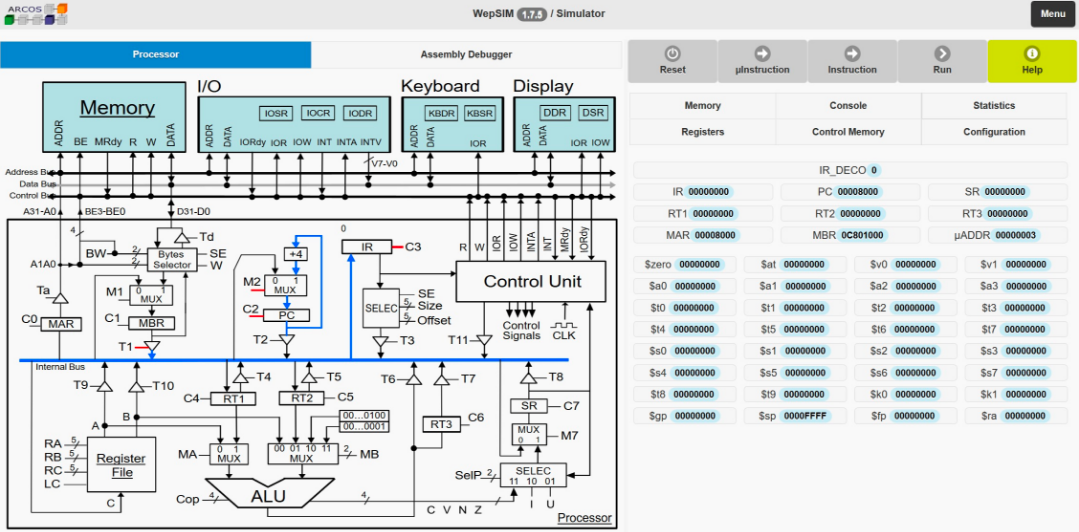
\includegraphics[width=15cm]{figures/anexob-9}
 	\caption{Pantalla principal: opciones para la ejecución.}
	\label{fig:anexob-9}
\end{figure}

Dando al botón ``Registers'' en la barra de botones situada en la parte superior derecha de la pantalla principal (Figura \ref{fig:anexob-9}) es posible ver cómo los valores de los registros son modificados durante la ejecución.

Es posible visualizar también la unidad de control como se muestra en la Figura \ref{fig:anexob-10}.

\begin{figure}[htbp]
 	\centering
 	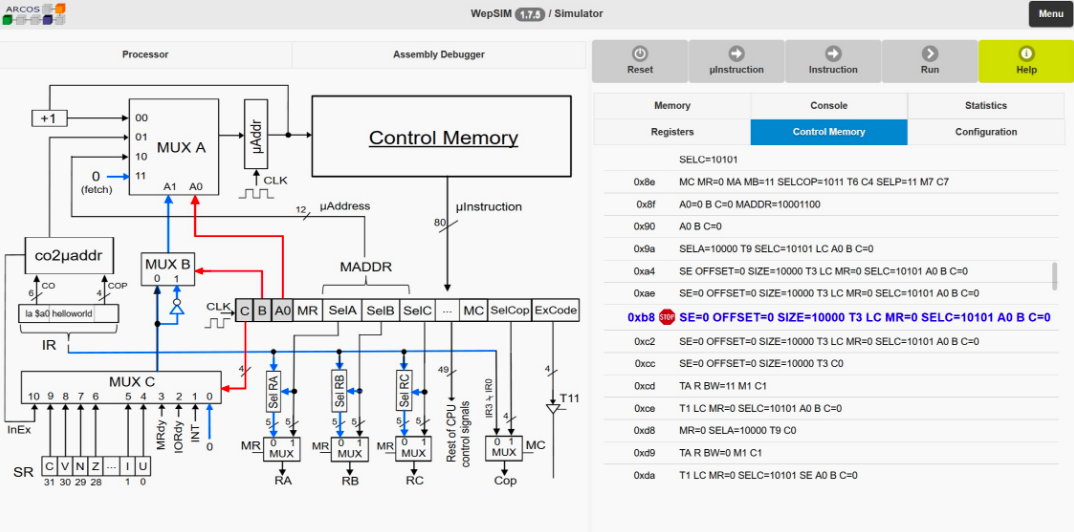
\includegraphics[width=15cm]{figures/anexob-10}
 	\caption{Pantalla principal: visualización de la unidad de control.}
	\label{fig:anexob-10}
\end{figure}

Así como también es posible reiniciar la ejecución haciendo clic al botón ``Reset'' situado en la barra de botones que aparece en la parte superior de la pantalla.

\section*{Formato del microcódigo}

El microcódigo se carga a través de un fichero de texto que tiene tres secciones:

\begin{itemize}

\item[1.] Lista de microprogramas.

\item[2.] Nombrado de registros.

\item[3.] Pseudo-instrucciones.

\end{itemize}

La lista de microprogramas comienza con el código del fetch. Un ejemplo de microprograma de fetch básico sería:

\begin{lstlisting}
begin
{
fetch: (T2, C0=1),
         (Ta, Td, R, BW=11, C1),
         (M2, C2, T1, C3),
         (A0, B=0, C=0000)
}
\end{lstlisting}

Las seńales de control situadas entre los paréntesis ( y ) se corresponden con las seńales a activar en un ciclo de reloj. Así el fetch necesita cuatro ciclos de reloj, el último se corresponde con la decodificación (incluida en dentro del fetch). A continuación se encuentran el resto de microprogramas asociados a cada instrucción. Cada microprograma sigue el siguiente formato:

\begin{lstlisting}
inst1 campo1 campo2 campo3
{
     co=000000,
     nwords=1,
     campo1=reg(25,21),
     campo2=reg(20,16),
     campo3=reg(15,11),
     {
         (Cop=1001, SelP=11, C7, T6, LC, SelA=10100, SelB=01111, SelC=10111,
          A0=1, B=1, C=0)
     }
}
\end{lstlisting}

Donde la primera línea describe el nombre de la instrucción (inst1) y los parámetros que tiene (registros, valores inmediatos, etc.). A continuación se abre un bloque con llaves para describir dicha instrucción.

El primer campo del ejemplo mostrado (co) indica los 6 bits que identifica unívocamente la instrucción. Esto no es del todo cierto para las instrucciones aritmético-lógicas puesto que es posible compartir el mismo código de operación y según el valor del campo cop diferenciarse. Un ejemplo de este caso sería:

\begin{lstlisting}
inst1 campo1 campo2 campo3
{
     co=000000,
     cop=0000,
     nwords=1,
     campo1=reg(25,21),
     campo2=reg(20,16),
     campo3=reg(15,11),
     {
         (Cop=1001, SelP=11, C7, T6, LC, SelA=10100, SelB=01111, SelC=10111,
          A0=1, B=1, C=0)
     }
}
\end{lstlisting}

Los siguientes campos indican para cada uno de los parámetros qué tipo es (registro, inmediato o dirección) así como el bit de inicio y final (valor de 0 a 31) entre los cuales está el valor de dicho parámetro. El tipo de parámetro se indica con:

\begin{itemize}

\item parametro1 = reg(bit-final, bit-inicio), para un registro, siendo los 5 bits que identifican el registro a usar.

\item parametro1 = inm(bit-final, bit-inicio), para un valor inmediato.

\item parametro1 = addr(bit-final, bit-inicio)rel, para una dirección relativa con respecto al PC.

\item parametro1 = addr(bit-final, bit-inicio)abs, para una dirección absoluta.

\end{itemize}

A continuación se abre un bloque donde se indicará el microprograma correspondiente a la instrucción. Las señales de cada ciclo están entre paréntesis y se separan dichos ciclos por coma. Si solo hay un ciclo no es necesario la coma. Dentro de los paréntesis se indicarán las señales y el valor correspondiente. Si es una señal de un bit, con solo poner el nombre de la señal se entenderá que su valor es uno. El valor de la señal se ha de indicar en binario, usando tantos bits como tenga asociado la señal. Las señales y su valor correspondientes se separan usando una coma. Para el nombrado de registros se precisa indicar la etiqueta que se usará para cada uno de los 32 registros del banco de registros. Un ejemplo de esta sección es:

\begin{lstlisting}
registers

{ 
	0=$zero, 
	1=$at, 
	2=$v0, 
	3=$v1, 
	4=$a0, 
	5=$a1, 
	6=$a2, 
	7=$a3, 
	. 
	. 
	. 
	24=$t8, 
	25=$t9, 
	26=$k0, 
	27=$k1, 
	28=$gp, 
	29=$sp (stack_pointer), 
	30=$fp, 
	31=$ra 
}
\end{lstlisting}

En la que se indican los nombres usados en la arquitectura MIPS32. En este ejemplo el registro 29 etiquetado con \$sp tiene el atributo ``(stack\_pointer)'' para indicar que será usado como puntero de pila.

Por último es posible definir pseudo-instrucciones. Un ejemplo de pseudoinstrucción sería:

\begin{lstlisting}
Pseudoinstructions
{
	li reg num
	{
		lui reg sel(31,16,num) ;
		ori reg reg sel(15,0,num)
	}
}
\end{lstlisting}

\section*{Formato del código ensamblador}

El código en ensamblador se describe en un fichero de texto con una primera sección de datos (.data) y una segunda sección para el código (.text).

En la sección de datos es posible definir las variables y constantes que se alojarán en el segmento de datos de la memoria principal. Dicha sección comienza con la directiva .data. Las directivas que permiten especificar los distintos tipos de datos que pueden definirse son:

\begin{itemize}
\item \textbf{.ascii:} va seguida de la cadena de caracteres, instruyendo al ensamblador para crear una zona de memoria con datos, y almacenar en ella la cadena que se indique.

\item \textbf{.asciiz:} va seguida de la cadena de caracteres, instruyendo al ensamblador para crear una zona de memoria con datos, y almacenar en ella la cadena que se muestra terminado por un byte con valor cero.

\item \textbf{.byte:} va seguida de uno o más valores que formarán parte del valor de la variable. En caso de varios valores, dichos valores se separarán por coma. Para los valores se puede usar: carácter, octal, hexadecimal y decimal.

\item \textbf{.half:} va seguida de uno o más valores que formarán parte del valor de la variable. En caso de varios valores, dichos valores se separarán por coma. Para los valores se puede usar: octal, hexadecimal y decimal.

\item \textbf{.word:} va seguida de uno o más valores que formarán parte del valor de la variable. En caso de varios valores, dichos valores se separarán por coma.
Para los valores se puede usar: octal, hexadecimal y decimal.

\item \textbf{.space:} va seguida del número de bytes, en formato decimal, que el usuario desea reservar en memoria.

\end{itemize}

El formato de un valor de los tipos de datos comentados es:

\begin{itemize}

\item \textbf{Cadena de caracteres:} secuencia de caracteres entre comillas dobles.\\
Por ejemplo: "hola 123\textbackslash n"

\item \textbf{Carácter:} carácter entre comillas simples.\\
Por ejemplo: 'c'.

\item \textbf{Octal:} un número que comienza por cero y sus dígitos son menores que ocho. \\
Por ejemplo: 012.

\item \textbf{Hexadecimal:} un número que comienza por el prefijo 0x y sus dígitos son del cero al nueve y las letras a, b, c, d, e y f.\\
Por ejemplo: 0x12.

\item \textbf{Decimal:} un número que no está en formato octal o hexadecimal con dígitos comprendidos entre el cero y el nueve (ambos incluidos).\\
Por ejemplo: 12.
\end{itemize}

En la sección de código es posible definir las subrutinas que se alojarán en el segmento de código de la memoria principal. Dicha sección comienza con la directiva .text.

Es posible usar comentarios de línea usando el carácter \#. Todo lo que hay a continuación de este carácter hasta el final de línea será ignorado por el ensamblador.

\vspace{4cm}

Un ejemplo programa sería:

\begin{lstlisting}
.data

	age1: .word 0x12345678, 20

	age2: .word 20 , 10

	resultado: .word 0

	# 32-bit word initialized with decimal

	texto: .ascii "Hola\t"

	texto2: .asciiz "Hola\t"

	hueco: .space 16

.text

.globl main

	main: li $3 2

	li $4 1

	li $5 0
\end{lstlisting}

\clearpage

\section*{Ejemplos}

\subsection*{Juego de instrucciones}

\begin{lstlisting}
begin
{
                    (A0=0, B=1, C=1, MADDR=fetch),
                    # push PC
                    (MR=1, SELA=11101, MA=0, MB=10, MC=1, SELCOP=1011, T6=1, SELC=11101, LC=1, C0),
                    (T2=1, M1=0, C1),
                    (BW=11, TA=1, TD=1, W=1)
                    # push SR
                    (MR=1, SELA=11101, MA=0, MB=10, MC=1, SELCOP=1011, T6=1, SELC=11101, LC=1, C0),
                    (T8=1, M1=0, C1),
                    (BW=11, TA=1, TD=1, W=1),
                    # MBR <- DB <- INTV
                    (INTA, BW=11, M1=1, C1=1),
                    # RT1 <- MBR
                    (T1=1, C4=1),
                    # MAR <- RT1*4
                    (MA=1, MB=10, MC=1, SELCOP=1100, T6, M2=0, C0),
                    # MBR <- MP[MAR]
                    (TA=1, R=1, BW=11, M1=1, C1=1),
                    # PC <- MAR
                    (T1, M2=0, C2),
    fetch:          (T2, C0),
                    (TA, R, BW=11, M1=1, C1=1),
                    (M2, C2, T1, C3),
                    (A0, B=0, C=0)
}



#
# INT
#

reti {
        co=111110,
        nwords=1,
        {
              # pop SR
              (MR=1, SELA=11101, T9, C0),
              (MR=1, SELA=11101, MA=0, MB=10, MC=1, SELCOP=1010, T6=1, SELC=11101, LC=1),
              (TA=1, R=1, BW=11, M1=1, C1),
              (T1=1, M7=0, C7),
              # pop PC
              (MR=1, SELA=11101, T9, C0),
              (MR=1, SELA=11101, MA=0, MB=10, MC=1, SELCOP=1010, T6=1, SELC=11101, LC=1),
              (TA=1, R=1, BW=11, M1=1, C1),
              (T1=1, M2=0, C2, A0=1, B=1 ,C=0)
        }
}


#
# ALU
#

and reg1 reg2 reg3 {
            co=000000,
            cop=0000,
            nwords=1,
            reg1=reg(25,21),
            reg2=reg(20,16),
            reg3=reg(15,11),
            {
                (MC=1, MR=0, SELA=1011, SELB=10000, MA=0, MB=0, SELCOP=1, T6=1, SELC=10101, LC=1, SELP=11, M7, C7, A0=1, B=1, C=0)
            }
}

or reg1 reg2 reg3 {
            co=000000,
            cop=0001,
            nwords=1,
            reg1=reg(25,21),
            reg2=reg(20,16),
            reg3=reg(15,11),
            {
                (MC=1, MR=0, SELA=1011, SELB=10000, MA=0, MB=0, SELCOP=10, T6=1, SELC=10101, LC=1, SELP=11, M7, C7, A0=1, B=1, C=0)
            }
}

not reg {
            co=000000,
            cop=0010,
            nwords=1,
            reg=reg(25,21),
            {
                (MC=1, MR=0, SELA=10101, MA=0, SELCOP=11, T6=1, SELC=10101, LC=1, SELP=11, M7, C7, A0=1, B=1, C=0)
            }
}

xor reg1 reg2 reg3 {
            co=000000,
            cop=0011,
            nwords=1,
            reg1=reg(25,21),
            reg2=reg(20,16),
            reg3=reg(15,11),
            {
                (MC=1, MR=0, SELA=1011, SELB=10000, MA=0, MB=0, SELCOP=100, T6=1, SELC=10101, LC=1, SELP=11, M7, C7, A0=1, B=1, C=0)
            }
}

add reg1 reg2 reg3 {
            co=000000,
            cop=1001,
            nwords=1,
            reg1=reg(25,21),
            reg2=reg(20,16),
            reg3=reg(15,11),
            {
                (MC=1, MR=0, SELA=1011, SELB=10000, MA=0, MB=0, SELCOP=1010, T6=1, SELC=10101, LC=1, SELP=11, M7, C7, A0=1, B=1, C=0)
            }
}

sub reg1 reg2 reg3 {
            co=000000,
            cop=1010,
            nwords=1,
            reg1=reg(25,21),
            reg2=reg(20,16),
            reg3=reg(15,11),
            {
                (MC=1, MR=0, SELB=1011, SELA=10000, MA=0, MB=0, SELCOP=1011, T6=1, SELC=10101, LC=1, SELP=11, M7, C7, A0=1, B=1, C=0)
            }
}

mul reg1 reg2 reg3 {
            co=000000,
            cop=1011,
            nwords=1,
            reg1=reg(25,21),
            reg2=reg(20,16),
            reg3=reg(15,11),
            {
                (MC=1, MR=0, SELA=1011, SELB=10000, MA=0, MB=0, SELCOP=1100, T6=1, SELC=10101, LC=1, SELP=11, M7, C7, A0=1, B=1, C=0)
            }
}

div reg1 reg2 reg3 {
            co=000000,
            cop=1100,
            nwords=1,
            reg1=reg(25,21),
            reg2=reg(20,16),
            reg3=reg(15,11),
            {
                (MC=1, MR=0, SELB=1011, SELA=10000, MA=0, MB=0, SELCOP=1101, T6=1, SELC=10101, LC=1, SELP=11, M7, C7, A0=1, B=1, C=0)
            }
}


#
# MV/L*
#

move reg1 reg2 {
            co=000001,
            nwords=1,
            reg1=reg(25,21),
            reg2=reg(20,16),
            {
                (SELA=10000, T9, SELC=10101, LC, A0=1, B=1, C=0)
            }
}

li reg val {
            co=000010,
            nwords=1,
            reg=reg(25,21),
            val=inm(15,0),
            {
                (SE=1, OFFSET=0, SIZE=10000, SE=1, T3=1, LC=1, MR=0, SELC=10101, A0=1, B=1, C=0)
            }
}

liu reg val {
            co=111100,
            nwords=1,
            reg=reg(25,21),
            val=inm(15,0),
            {
                (SE=1, OFFSET=0, SIZE=10000, SE=0, T3=1, LC=1, MR=0, SELC=10101, A0=1, B=1, C=0)
            }
}

la  reg addr {
            co=000011,
            nwords=1,
            reg=reg(25,21),
            addr=address(15,0)abs,
            {
                (SE=0, OFFSET=0, SIZE=10000, T3=1, LC=1, MR=0, SELC=10101, A0=1, B=1, C=0)
            }
}

la  reg addr {
            co=111111,
            nwords=2,
            reg=reg(25,21),
            addr=address(63,32)abs,
            {
                (SE=0, OFFSET=0, SIZE=10000, T3=1, LC=1, MR=0, SELC=10101, A0=1, B=1, C=0)
            }
}

lw reg addr {
            co=000100,
            nwords=1,
            reg=reg(25,21),
            addr=address(15,0)abs,
            {
                (SE=0, OFFSET=0, SIZE=10000, T3=1, C0=1),
                (TA=1, R=1, BW=11, M1=1, C1=1),
                (T1=1, LC=1, MR=0, SELC=10101, A0=1, B=1, C=0)
            }
}

lb reg1 (reg2) {
            co=100101,
            nwords=1,
            reg1 = reg(25,21),
            reg2 = reg(20,16),
            {
                (MR=0, SELA=10000, T9=1, C0),
                (TA=1, R=1, BW=00, M1=1, C1=1),
                (T1=1, LC=1, MR=0, SELC=10101, SE=1, A0=1, B=1, C=0)
            }
}

lbu reg1 (reg2) {
            co=101111,
            nwords=1,
            reg1 = reg(25,21),
            reg2 = reg(20,16),
            {
                (MR=0, SELA=10000, T9=1, C0),
                (TA=1, R=1, BW=00, M1=1, C1=1),
                (T1=1, LC=1, MR=0, SELC=10101, SE=0, A0=1, B=1, C=0)
            }
}

lw reg1 (reg2)
{
            co=100000,
            nwords=1,
            reg1 = reg(25,21),
            reg2 = reg(20,16),
            {
                (MR=0, SELA=10000, T9, C0),
                (TA=1, R=1, BW=11, M1=1, C1=1),
                (T1=1, LC=1, MR=0, SELC=10101, A0=1, B=1, C=0)
            }
}

sw reg addr {
            co=000101,
            nwords=1,
            reg=reg(25,21),
            addr=address(15,0)abs,
            {
                (SE=0, OFFSET=0, SIZE=10000, T3=1, C0=1),
                (MR=0, SELA=10101,    T9=1, M1=0, C1=1),
                (BW=11, TA=1, TD=1,     W=1,  A0=1, B=1, C=0)
            }
}

lb reg addr {
            co=001000,
            nwords=1,
            reg=reg(25,21),
            addr=address(15,0)abs,
            {
                (SE=0, OFFSET=0, SIZE=10000, T3=1, C0=1),
                (TA=1, R=1, BW=00, SE=1, M1=1, C1=1),
                (T1=1, LC=1, MR=0, SELC=10101, A0=1, B=1, C=0)
            }
}

sb reg addr {
            co=001001,
            nwords=1,
            reg=reg(25,21),
            addr=address(15,0)abs,
            {
                (SE=0, OFFSET=0, SIZE=10000, T3=1, C0=1),
                (MR=0, SELA=10101,    T9=1, M1=0, C1=1),
                (BW=0, TA=1, TD=1,     W=1,  A0=1, B=1, C=0)
            }
}


#
# IN/OUT
#

in reg val {
            co=001010,
            nwords=1,
            reg=reg(25,21),
            val=inm(15,0),
            {
                (SE=0, OFFSET=0, SIZE=10000, T3=1, C0=1),
                (TA=1, IOR=1,    M1=1, C1=1),
                (T1=1, LC=1,     MR=0, SELC=10101, A0=1, B=1, C=0)
            }
}

out reg val {
            co=001011,
            nwords=1,
            reg=reg(25,21),
            val=inm(15,0),
            {
                (SE=0, OFFSET=0, SIZE=10000, T3=1, C0=1),
                (MR=0, SELA=10101, T9=1,    M1=0, C1=1),
                (TA=1, TD=1,     IOW=1,   A0=1, B=1, C=0)
            }
}


#
# b*
#

b offset {
            co=001100,
            nwords=1,
            offset=address(15,0)rel,
            {
                (T2, C4),
                (SE=1, OFFSET=0, SIZE=10000, T3, C5),
                (MA=1, MB=1, MC=1, SELCOP=1010, T6, C2, A0=1, B=1, C=0)
            }
}

beq reg reg offset {
            co=001101,
            nwords=1,
            reg=reg(25,21),
            reg=reg(20,16),
            offset=address(15,0)rel,
            {
                (T8, C5),
                (SELA=10101, SELB=10000, MC=1, SELCOP=1011, SELP=11, M7, C7),
                (A0=0, B=1, C=110, MADDR=bck2ftch),
                (T5, M7=0, C7),
                (T2, C4),
                (SE=1, OFFSET=0, SIZE=10000, T3, C5),
                (MA=1, MB=1, MC=1, SELCOP=1010, T6, C2, A0=1, B=1, C=0),
      bck2ftch: (T5, M7=0, C7),
                (A0=1, B=1, C=0)
            }
}

bne reg reg offset {
            co=001110,
            nwords=1,
            reg=reg(25,21),
            reg=reg(20,16),
            offset=address(15,0)rel,
            {
                (T8, C5),
                (SELA=10101, SELB=10000, MC=1, SELCOP=1011, SELP=11, M7, C7),
                (A0=0, B=0, C=110, MADDR=bck3ftch),
                (T5, M7=0, C7),
                (T2, C4),
                (SE=1, OFFSET=0, SIZE=10000, T3, C5),
                (MA=1, MB=1, MC=1, SELCOP=1010, T6, C2, A0=1, B=1, C=0),
      bck3ftch: (T5, M7=0, C7),
                (A0=1, B=1, C=0)
            }
}

bge reg reg offset {
            co=001111,
            nwords=1,
            reg=reg(25,21),
            reg=reg(20,16),
            offset=address(15,0)rel,
            {
                (T8, C5),
                (SELA=10101, SELB=10000, MC=1, SELCOP=1011, SELP=11, M7, C7),
                (A0=0, B=0, C=111, MADDR=bck4ftch),
                (T5, M7=0, C7),
                (T2, C4),
                (SE=1, OFFSET=0, SIZE=10000, T3, C5),
                (MA=1, MB=1, MC=1, SELCOP=1010, T6, C2, A0=1, B=1, C=0),
      bck4ftch: (T5, M7=0, C7),
                (A0=1, B=1, C=0)
            }
}

blt reg reg offset {
            co=010000,
            nwords=1,
            reg=reg(25,21),
            reg=reg(20,16),
            offset=address(15,0)rel,
            {
                (T8, C5),
                (SELA=10101, SELB=10000, MC=1, SELCOP=1011, SELP=11, M7, C7),
                (A0=0, B=1, C=111, MADDR=bck5ftch),
                (T5, M7=0, C7),
                (T2, C4),
                (SE=1, OFFSET=0, SIZE=10000, T3, C5),
                (MA=1, MB=1, MC=1, SELCOP=1010, T6, C2, A0=1, B=1, C=0),
      bck5ftch: (T5, M7=0, C7),
                (A0=1, B=1, C=0)
            }
}

bgt reg reg offset {
            co=010001,
            nwords=1,
            reg=reg(25,21),
            reg=reg(20,16),
            offset=address(15,0)rel,
            {
                (T8, C5),
                (SELA=10101, SELB=10000, MC=1, SELCOP=1011, SELP=11, M7, C7),
                (A0=0, B=0, C=111, MADDR=bck6ftch),
                (A0=0, B=0, C=110, MADDR=bck6ftch),
                (T5, M7=0, C7),
                (T2, C4),
                (SE=1, OFFSET=0, SIZE=10000, T3, C5),
                (MA=1, MB=1, MC=1, SELCOP=1010, T6, C2, A0=1, B=1, C=0),
      bck6ftch: (T5, M7=0, C7),
                (A0=1, B=1, C=0)
            }
}

ble reg reg offset {
            co=010010,
            nwords=1,
            reg=reg(25,21),
            reg=reg(20,16),
            offset=address(15,0)rel,
            {
                (T8, C5),
                (SELA=10101, SELB=10000, MC=1, SELCOP=1011, SELP=11, M7, C7),
                (A0=0, B=0, C=111, MADDR=ble_ys),
                (A0=0, B=0, C=110, MADDR=ble_ys),
                (T5, M7=0, C7),
                (A0=1, B=1, C=0),
        ble_ys: (T5, M7=0, C7),
                (T2, C4),
                (SE=1, OFFSET=0, SIZE=10000, T3, C5),
                (MA=1, MB=1, MC=1, SELCOP=1010, T6, C2, A0=1, B=1, C=0)
            }
}


#
# j*
#

j addr {
            co=010011,
            nwords=1,
            addr=address(15,0)abs,
            {
                (SE=0, OFFSET=0, SIZE=10000, T3=1, M2=0, C2=1, A0=1, B=1, C=0)
            }
}

jal addr {
            co=010100,
            nwords=1,
            addr=address(15,0)abs,
            {
                (T2, SELC=11111, MR=1, LC),
                (SE=0, OFFSET=0, SIZE=10000, T3=1, M2=0, C2=1, A0=1, B=1, C=0)
            }
}

jr reg1 {
            co=010101,
            nwords=1,
            reg1=reg(25,21),
            {
                (SELA=10101, T9=1, C2=1, A0=1, B=1, C=0)
            }
}


#
# Misc
#

nop {
        co=010110,
        nwords=1,
        {
                (A0=1, B=1, C=0)
        }
}

srl reg1 reg2 val {
            co=010111,
            nwords=1,
            reg1=reg(25,21),
            reg2=reg(20,16),
            val=inm(5,0),
            {
                (SE=1, OFFSET=0, SIZE=110, T3=1, C4=1),
                (MC=1, MR=0, SELA=10000, SELB=10000, MA=0, MB=0, SELCOP=1, T6=1, SELC=10101),
         loop9: (A0=0, B=0, C=110, MADDR=bck2ftch),
                (MC=1, MR=0, SELA=10101, SELB=10101, MA=0, MB=0, SELCOP=101, T6=1, LC=1, SELC=10101),
                (MC=1, MR=0, MA=1, MB=11, SELCOP=1011, T6=1, C4=1, SELP=11, M7, C7),
                (A0=0, B=1, C=0, MADDR=loop9),
      bck9ftch: (A0=1, B=1, C=0)
            }
}


registers
{
        0=$zero,
        1=$at,
        2=$v0,
        3=$v1,
        4=$a0,
        5=$a1,
        6=$a2,
        7=$a3,
        8=$t0,
        9=$t1,
        10=$t2,
        11=$t3,
        12=$t4,
        13=$t5,
        14=$t6,
        15=$t7,
        16=$s0,
        17=$s1,
        18=$s2,
        19=$s3,
        20=$s4,
        21=$s5,
        22=$s6,
        23=$s7,
        24=$t8,
        25=$t9,
        26=$k0,
        27=$k1,
        28=$gp,
        29=$sp (stack_pointer),
        30=$fp,
        31=$ra
}

pseudoinstructions
{
	lii reg num 
        {	
            li reg sel(31,16,num) ; 
            li reg sel(15,0,num) 
        }

}
\end{lstlisting}

\clearpage

\subsection*{Código ensamblador}

\begin{lstlisting}

.data

   matrix: .word 1, 0, 3, 0, 0, 1
           .word 1, 2, 0, 1, 1, 0

.text

counting:
       # result = 0
       li   $v0 0

       # for ($t0=0; $t0 < $a1; ...
       li   $t0 0
   b1: bge  $t0 $a1 f1

       # for ($t1=0; $t1 < $a2; ...
       li   $t1 0
   b2: bge  $t1 $a2 f2

       # $t2 = ($t0*$a2 + $t1) * 4
       mul  $t2 $t0 $a2
       add  $t2 $t2 $t1
       li   $t3 4
       mul  $t2 $t2 $t3

       # elto = *( $a0 + $t2 ) 
       add  $t2 $a0 $t2
       lw   $t2 ($t2)

       bne  $t2 $0 nozero
       li   $t3 1
       add  $v0 $v0 $t3
nozero: 

       # ... $t1++) 
       li   $t3 1
       add  $t1 $t1 $t3
       b b2

f2:
       # ... $t0++) 
       li   $t3 1
       add  $t0 $t0 $t3
       b b1

f1:
       # return
       jr $ra


main: 
       # counting (matrix, 2, 6)
       la  $a0 matrix
       li  $a1 2
       li  $a2 6
       jal counting


\end{lstlisting}